\documentclass[a4paper,oneside,12pt]{book}

%----------------------------------------------------------------------------------------
%	README!
%   Welcome. It's worth having a read through this file
%   to set up the broad parameters, such as the name of
%   the degree, the school/department, the type of work
%   (dissertation/Final Year Project/report, etc. as well
%   as your details.
%----------------------------------------------------------------------------------------

%----------------------------------------------------------------------------------------
%	COVER PAGE
%   The cover page is laid out in title/title.tex. You can choose a color
%   or black and white logo
%----------------------------------------------------------------------------------------

%----------------------------------------------------------------------------------------
%	THESIS INFORMATION
%   Put title, author name, supervisor name, degree, type of work, school, department in here
%   It will be used for the title page and the embedded PDF information
%----------------------------------------------------------------------------------------

\newcommand{\thesistitle}{Parallelizing the Conjugate Gradient Method with MPI} % Your thesis title, this is used in the title and abstract
\newcommand{\degree}{MAI (Computational Science and Engineering)} % Replace with your degree name, this is used in the title page and abstract
\newcommand{\typeofthesis}{MATH-454 Assignment 1} % dissertation, Final Year Project, report, etc.
\newcommand{\authorname}{Aaron Dinesh} % Your name, this is used in the title page and PDF stuff
%% Do not put your Student ID in the document, as TCD will not publish
%% documents that contain both your name and your Student ID.
\newcommand{\supervisor}{} % replace with the name of your supervisor
%\newcommand{\cosupervisor}{Dr. Alex Lee} % replace with the name of your co-supervisor if you have one
\newcommand{\keywords}{} % Replace with keywords for your thesis
\newcommand{\school}{} % Your school's name and URL, this is used in the title page
%Edited by HS for engineering

%% Comment out the next line if you don't want a department to appear
\newcommand{\department}{} % Your research group's name and URL, this is used in the title page


%% Language and font encodings
\usepackage[T1]{fontenc} 
\usepackage[utf8]{inputenc}
\usepackage[english]{babel}
\usepackage{ulem}
%% Bibliographical stuff
\usepackage[]{cite}
%% Document size
%Include showframe as an option if you want to see the boxes
\usepackage[a4paper,top=2.54cm,bottom=2.54cm,left=2.54cm, right=2.54cm,headheight=16pt]{geometry}
\setlength{\marginparwidth}{2cm}
%% Useful packages
\usepackage{amsmath}
\usepackage{amsfonts}
\usepackage{dsfont}
\usepackage[autostyle=true]{csquotes} % Required to generate language-dependent quotes in the bibliography
\usepackage[pdftex]{graphicx}
\usepackage[colorinlistoftodos]{todonotes}
\usepackage[colorlinks=true, allcolors=black]{hyperref}
\usepackage{hyperxmp}
\usepackage{caption} % if no caption, no colon
\usepackage{sfmath} %use sans-serif in the maths sections too
\usepackage[parfill]{parskip}    % Begin paragraphs with an empty line rather than an indent
\usepackage{setspace} % to permit one-and-a-half or double spacing
\usepackage{enumerate} % fancy enumerations like (i) (ii) or (a) (b) and such
\usepackage{booktabs} % To thicken table lines
\usepackage{fancyhdr}
\usepackage{xcolor} % to get TCD color on headings
\usepackage{hvfloat}
\usepackage{listings}
\usepackage{subcaption}
\usepackage{placeins}
\usepackage{xargs}                      % Use more than one optional parameter in a new commands
\usepackage{tikz}
\usepackage{diagbox}  % Required for diagonal split
\usepackage{booktabs}
\usetikzlibrary{datavisualization}
\usetikzlibrary{datavisualization.formats.functions}
\usetikzlibrary{datavisualization}


\hbadness=10000
\captionsetup[figure]{font={default, sf}}
\setcounter{tocdepth}{4}
\graphicspath{{./Images/}}
\numberwithin{equation}{chapter} %HS edit for (chapter.equation)
\pagestyle{plain} % Embrace simplicity!
\counterwithout{figure}{section}
\definecolor{tcd_blue}{RGB}{5, 105, 185}
\newcommandx{\change}[2][1=]{\todo[linecolor=blue,backgroundcolor=blue!25,bordercolor=blue,#1]{#2}}

%% For Today's Date
\renewcommand{\today}{\ifnum\number\day<10 0\fi \number\day \space%
\ifcase \month \or January\or February\or March\or April\or May%
\or June\or July\or August\or September\or October\or November\or December\fi \space%
\number \year}

%% Defining Code Colors
\definecolor{codegreen}{rgb}{0,0.6,0}
\definecolor{codegray}{rgb}{0.5,0.5,0.5}
\definecolor{codepurple}{rgb}{0.58,0,0.82}
\definecolor{backcolour}{rgb}{0.95,0.95,0.92}
\definecolor{epfl_red}{RGB}{255, 0, 0}

\lstdefinestyle{codeStyle}{
    backgroundcolor=\color{backcolour},   
    commentstyle=\color{codegreen},
    keywordstyle=\color{magenta},
    numberstyle=\tiny\color{codegray},
    stringstyle=\color{codepurple},
    basicstyle=\ttfamily\footnotesize,
    breakatwhitespace=false,         
    breaklines=true,                 
    captionpos=b,                    
    keepspaces=true,                 
    numbers=left,                    
    numbersep=5pt,                  
    showspaces=false,                
    showstringspaces=false,
    showtabs=false,                  
    tabsize=2
}

\lstset{style=codeStyle}

\lstdefinelanguage{Julia}%
  {morekeywords={abstract,break,case,catch,const,continue,do,else,elseif,%
      end,export,false,for,function,immutable,import,importall,if,in,%
      macro,module,otherwise,quote,return,switch,true,try,type,typealias,%
      using,while,struct,mutable},%
   sensitive=true,%
   alsoother={\$},%
   morecomment=[l]\#,%
   morecomment=[n]{\#=}{=\#},%
   morestring=[s]{"}{"},%
   morestring=[m]{'}{'},%
}[keywords,comments,strings]%

\lstset{%
    language         = Julia,
    basicstyle       = \ttfamily,
    keywordstyle     = \bfseries\color{magenta},
    stringstyle      = \color{codepurple},
    commentstyle     = \color{codegreen},
    showstringspaces = false,
}



%% It's personal taste but...
%% Uncomment the following block if you want your name and ID at the top of
%% (almost) every page.

%\pagestyle{fancy}
%\fancyhf{} % sets both header and footer to nothing
%\renewcommand{\headrulewidth}{0pt}
%\cfoot{\thepage}
%\ifdefined\authorid
%\chead{\it \authorname\ (\authorid)}
%\else
%\chead{\it \authorname}
%\fi
%% End of block

%% It is good practice to make your font sans-serif to improve the accessibility of your document.  Comment out the following line to disable it (but you really should not)
\renewcommand{\familydefault}{\sfdefault} %use the sans-serif font as default

%% If you insist on not using sans-serif (please don't), consider using Palatino instead of the LaTeX standard
%\usepackage{mathpazo} % Use the Palatino font by default if you prefer it to Computer Modern


%% Format Chapter headings appropriately
\usepackage{titlesec}
\titleformat{\chapter}[hang]{\normalfont\huge\bfseries\color{epfl_red}}{\thechapter}{1cm}{}{}
\titleformat{\section}{\color{epfl_red}\normalfont\Large\bfseries}{\color{epfl_red}\thesection}{1em}{}
\title{\thesistitle}
\author{\authorname}

\hypersetup{
   pdftitle=\thesistitle, % Set the PDF's title to your title
   pdfauthor=\authorname, % Set the PDF's author to your name
   pdfkeywords=\keywords, % Set the PDF's keywords to your keywords
   pdfsubject=\degree, % Set the PDF's keywords to your keywords
   pdfinfo={
     pdfsupervisor=\supervisor, % Set the PDF's supervisor to your supervisor
     %pdfcosupervisor=\cosupervisor, % Set the PDF's cosupervisor to your cosupervisor if using
   }
}


\frontmatter
\begin{document}

\begin{titlepage}

\center % Center everything on the page

%% All the text parameters should be taken from the start of the main.tex file.
%% You should only alter stuff here if you want to change the layout

%----------------------------------------------------------------------------------------
%	LOGO SECTION
%----------------------------------------------------------------------------------------
%% Choose one of the following -- a colour or black-and-white logo
\begin{figure*}
    \centering
    
\includegraphics[width=0.7\textwidth]{EPFL_Logo_Digital_RGB_PROD.png}\\[1cm] 
\end{figure*}
%\includegraphics[width=12cm]{title/black-stacked-trinity.jpg}\\[1cm] 


%----------------------------------------------------------------------------------------
%	TITLE SECTION
%----------------------------------------------------------------------------------------
\makeatletter
{ \huge \bfseries \thesistitle}\\[1.5cm] % Title of your document
 

%----------------------------------------------------------------------------------------
%	AUTHOR SECTION
%----------------------------------------------------------------------------------------

\ifdefined\authorid
\authorname\\ % Your name
\authorid\\[2cm] % Your Student ID
\else
\authorname\\[2cm] % Your name
\fi

%----------------------------------------------------------------------------------------
%	Supervisor SECTION
%----------------------------------------------------------------------------------------


%----------------------------------------------------------------------------------------
%	DATE SECTION
%----------------------------------------------------------------------------------------

{\large \today}\\[2cm] % Date, change the \today to a set date if you want to be precise

 
%----------------------------------------------------------------------------------------
%	TYPE OF THESIS SECTION
%----------------------------------------------------------------------------------------
\vfill
 A project submitted in fulfilment\\of the requirements for MATH-454

\vfill % Fill the rest of the page with whitespace

\end{titlepage}
\pagenumbering{roman}
\section*{\Huge\textcolor{epfl_red}{Declaration}}
I hereby declare that this work is fully my own.
\vspace{1cm}

Signed: \uline{\hfill Aaron Dinesh \hfill} Date: \uline{\hfill \today \hfill}

\newpage

%%\section*{\Huge\textcolor{tcd_blue}{Nomenclature}}
%%\begin{tabular}{lp{9cm}l}
%%  A        & Area of the wing                                                               & $m^{2}$ \\
%%  B                                                                                                   \\
%%  C        & Roman letters first, with capitals\ldots                                                 \\
%%  a        & then lower case.                                                                         \\
%%  b                                                                                                   \\
%%  c                                                                                                   \\
%%  $\Gamma$ & Followed by Greek capitals\ldots                                                         \\
%%  $\alpha$ & then lowercase Greek symbols.                                                           \\
%%  $\beta$                                                                                             \\
%%  $\epsilon$                                                                                          \\
%%  TLA      & Finally, three letter acronyms and other abbreviations arranged alphabetically           \\
%%\end{tabular}
%%\vspace{2cm}
%%
%%If a parameter has a typical unit that is used throughout your report, then it should be included here on the right hand side.
%%
%%If you have a very mathematical report, then you may wish to divide the nomenclature list into functions and variables, and then sub- and super-scripts.
%%
%%If you have a large number of acronyms, check out \href{https://www.overleaf.com/learn/latex/Glossaries} to make that more robust.
%%
%%Note that Roman mathematical symbols are typically in a serif font in italics.

\mainmatter
% Maintaining separate .tex files for each chapter is good practice
\setcounter{chapter}{1}
\section{Introduction}
In this assignment, a serial implementation of the Conjugate Gradient Method (CGM) was provided, which required
parallelization. In order to parallelize this implementation OpenMPI and the MPI parallelization paradigm was used.

\section{Serial Analysis}
The serial implementation of the CGM was evaluated using the provided \lstinline[language=C]|lap2D_5pt_n1000.mtx| matrix. This matrix
was chosen as its large size allowed for obvious parallelization opportunities to be revealed. The \lstinline[language=C]|perf|
profiling tool was used to analyse the serial code's execution time. From the profiling results, the \lstinline[language=C]|mat_vec|
function was identified as the primary computational bottleneck, accounting for approximately 86.27\% of the total execution
time. Consequently, the serial fraction of the program was estimated to be 13.73\%. The testing for the serial and
parallel code were performed on the Jed Cluster with and Intel Xeon Platinum 8360Y CPU, running at  2.40 GHz.


These values along with Amdahl's and Gustafson's laws for strong and weak scaling were used to calculate a theoretical
upper bound on the possible speed-ups that could be achieved using parallelization. The speed-ups were calculated using
the following equations~\cite{AmdahlGustafson2023}: 
\begin{align*}
   \text{Amdahl's Law (Strong Scaling)} = \frac{1}{(1-\alpha) + \frac{\alpha}{p}} 
\end{align*}
Here $\alpha$ is the fraction of the code that can be parallelized and $p$ is the number of processors. Gustafson's
equations are as follows:
\begin{align*}
    \text{Gustafson's Law (Weak Scaling)} = (1-\alpha) + \alpha p 
\end{align*}

\begin{figure}[h!]
    \centering
    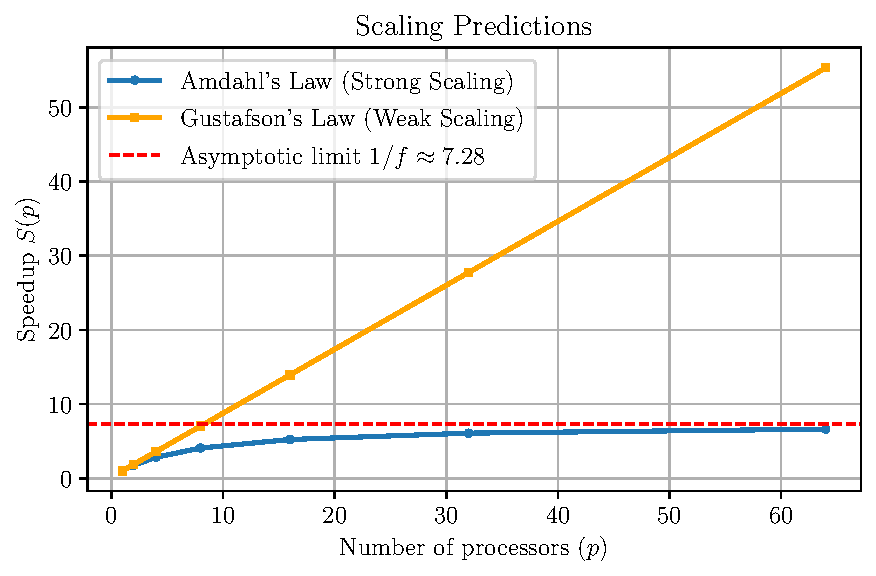
\includegraphics[width=\textwidth]{plots/scaling_laws.pdf}
    \caption{Strong and Weak Scaling Analysis using Amdahl's and Gustafson's Laws}
    \label{fig:AmdahlPlot}
\end{figure}
\FloatBarrier

\section{Parallel Modifications}
In order to parallelize the code with the least amount of communications, it was decided that the best course of action
would be to read in the matrix on processor 0 and then block distribute the row index, column index and value array to
each processor. Doing this when reading the matrix would implicitly parallelize the \lstinline[language=C]|mat_vec|
function and would reduce the communication needed to requiring just one \lstinline[language=C]|MPI_Allgather| after
each call to \lstinline[language=C]|mat_vec|, rather than a \lstinline[language=C]|MPI_Scatterv| and a
\lstinline[language=C]|MPI_Allgather| before and after the \lstinline[language=C]|mat_vec| calls. MPI message
packing and unpacking were also used to speed up this initial data transfer. This was enough to show some initial
improvements over the serial execution of the code, however, there was a lot more that could be done in the
\lstinline[language=C]|CGSolverSparse::solve()| function to further improve the parallelization of the code. Further
optimization was achieved through the use non-blocking transfers such as \lstinline[language=C]|MPI_Iallgatherv| as
well as combined communications such as \lstinline[language=C]|MPI_Reduce_scatter|. Using these combined
communications allows the MPI compiler to perform further optimizations when compiling the code. I also made use of
cblas operations such as \lstinline[language=C]|cblas_dcopy|, \lstinline[language=C]|cblas_daxpy| and
\lstinline[language=C]|cblas_ddot| to make use of the optimized implementations in the cblas library.

\section{Parallel Performance}
It was expected that the modifications introduced to the codebase would result in an improvement over sequential
runtimes. However, experimental results did not support this assumption. During testing, the parallel implementation
demonstrated poor scaling behaviour on the Jed Cluster. To illustrate this, strong and weak scaling experiments were
conducted. For Strong Scaling, the matrix \lstinline[language=C]|lap2D_5pt_n1000.mtx| and \lstinline[language=C]|lap2D_5pt_n200.mtx| were used, with the processor
counts ranging from 1 to 64 in powers of 2. The upper limit of 64 was selected based on the fact that no meaningful
scaling was observed past this point. In most configurations, the parallel solver performed comparably to the serial
implementation however in some cases, performance was slightly worse. The speed-up in the strong scaling case was
calculated using the following formula:
\begin{equation*}
    S(p) = \frac{T_1}{T_p}
\end{equation*}

where the subscript denotes the number of processors used. For the weak scaling experiments, the run time of a single
processor was tested with the \lstinline[language=C]|lap2D_5pt_n100.mtx| matrix. Then the processor count was raised
in powers of 2 and they were tested against the other matrices provided. From these experiments the runtime and the
iteration count to convergence were calculated. The speed-up in the weak scaling case is then calculated as follows:
\begin{equation*}
    S(p) = \frac{T_1 / I_1}{T_p / I_p}    
\end{equation*}

Where $I_{p}$ is the iteration count to convergence for $p$ processors. Since weak scaling requires the work done at
each test to be constant, the runtime was divided by the iteration count. The results form these experiments are shown
in the graphs below.

\begin{figure}[h!]
    \centering
    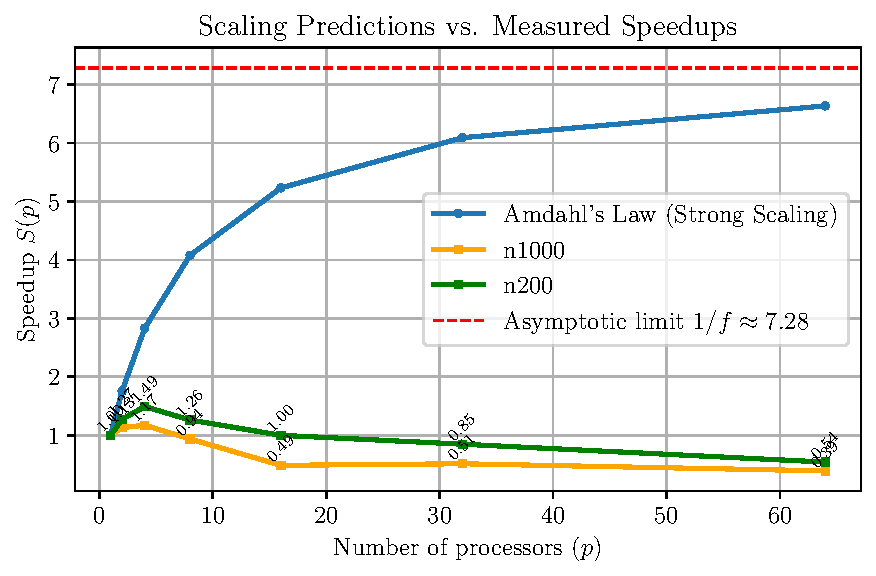
\includegraphics[width=\textwidth]{plots/strong_scaling.pdf}
    \caption{Strong Scaling Analysis}
    \label{fig:StrongScaling}
\end{figure}
\FloatBarrier

As can be seen from the graph above, minor performance gains can be achieved by switching from a serial code to a few
parallel processes. However, past 8 processors no further improvements are observed. A similar story can also be seen
when performing a weak scaling analysis, as can be seen in the graph below. \\

\begin{figure}[h!]
    \centering
    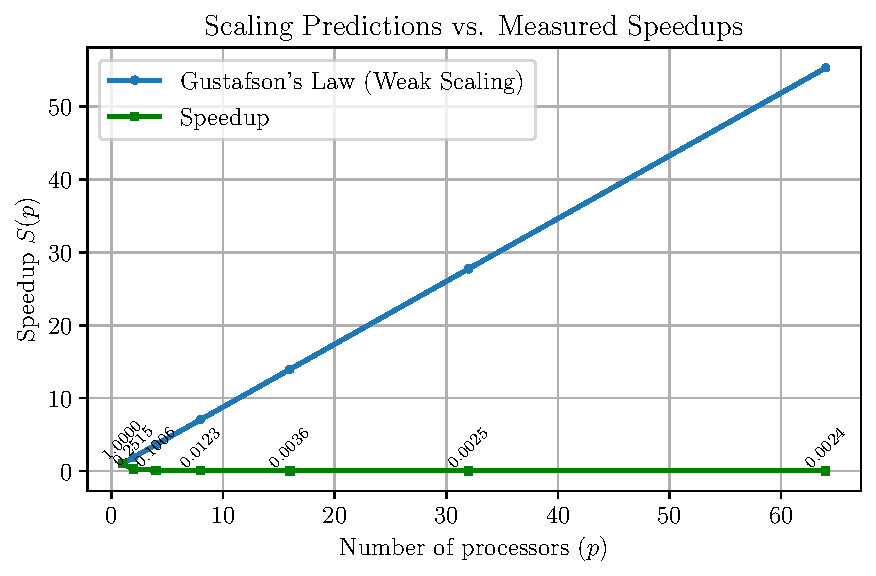
\includegraphics[width=\textwidth]{plots/weak_scaling.pdf}
    \caption{Weak Scaling Analysis}
    \label{fig:WeakScaling}
\end{figure}
\FloatBarrier

The raw results of the strong and weak scaling analysis can be seen in the tables below. \\

\begin{table}[h!]
    \centering
    \begin{tabular}{|c|c|c|c|c|c|c|c|}
        \hline
        \diagbox{Matrix Size}{\# Procs} & 1 & 2 & 4 & 8 & 16 & 32 & 64 \\ \hline
        n200 & 1.00 & 1.13 & 1.17 & 0.94 & 0.49 & 0.51 & 0.39 \\ \hline
        n1000 & 1.00 & 1.27 & 1.49 & 1.26 & 1.00 & 0.85 & 0.54 \\ \hline
    \end{tabular}
    \caption{Strong scaling speedup for different matrix sizes}
\end{table}

        
% weak scaling speed up data [1. 0.25147243 0.10058002 0.0122578  0.00355457 0.00252197 0.00238294]

\begin{table}[h!]
    \centering
    \begin{tabular}{|c|c|c|c|c|c|c|c|}
        \hline
        \# Procs & 1 & 2 & 4 & 8 & 16 & 32 & 64 \\ \hline
        speedup & 1. & 0.25147243 & 0.10058002 & 0.0122578 & 0.00355457 & 0.00252197 & 0.00238294 \\ \hline
    \end{tabular}
    \caption{Weak scaling speedup}
\end{table}

It is suspected that the small initial performance gains observed in the strong and weak scaling analysis are primarily
due to the distribution of the sparse matrix across all participating processors, allowing for some performance gains in
the \lstinline[language=C]|mat_vec| function. However, this advantage is quickly overshadowed by the substantial
cost incurred by the collective communication required to calculate the full matrix vector product. As the
dimensionality of the system increases the volume of data involved in these collectives grows correspondingly, leading
to significant communication latency that dominates in the overall runtime, especially when considering strong scaling.
\\
To address this issue, several mitigation strategies were explored. The first made use of non-blocking communications
such as \lstinline[language=C]|MPI_Iallreduce|, to allow for independent work to be completed while the communication continued in the
background. While this yielded some improvements, the gains were minor due to the relatively tight coupling between
global reductions and subsequent computations. The second made significant use of optimized BLAS functions. The
reasoning behind this was that the BLAS functions were optimized for operations on large vectors and matrices. However,
as was the case before, the performance gains were minor, yielding further credibility to the idea that that main
bottleneck is the communication overhead. \\
A more effective solution, however, would be to make use of modified CG algorithms that are better suited for parallel
execution. For example the Global Reduction pipelining CG algorithm proposed by Cool and Cornelis et al.
\cite{cools2019improvingstrongscalingconjugate} reformulates the classic CG iteration to allow for multiple operations
to be overlapped with global communication. They introduce an auxiliary Krylov basis and structure the algorithm to
delay the use of reduction results by $\ell$ iterations, allowing them to overlap $\ell$ operations with a single
\lstinline[language=C]|MPI_Iallreduce| call. Through the use of this algorithm, the team demonstrates strong scaling
results up to 1024 nodes with 16 MPI ranks per node on the US Department of Energy's NERSC ``Cori'' machine.
% note that your supervisor may have a strong opinion on the style of referencing you use. Some background is available at https://www.overleaf.com/learn/latex/Bibtex_bibliography_styles
\bibliographystyle{IEEEtran} %Changed to IEEETran by HS
%\bibliographystyle{unsrt}

\bibliography{citations.bib}
\appendix
\renewcommand{\thechapter}{A\arabic{chapter}}


\end{document}